%==============================================================
%  МАТЕМАТИК АНАЛИЗ I — ЛЕКЦ 4: Функцийн ойлголт ба ангилал, олон гишүүнт ба рационал функц
%--------------------------------------------------------------
%  Зөвхөн биеийн хэсэг. Таны преамбул дахь \itcol, definition, theorem,
%  example, remark, problem, solution, prof орчнууд болон tikz, pgfplots,
%  enumitem, amsmath, amssymb-ийг ашиглана.
%==============================================================
\providecommand{\R}{\mathbb{R}}
\providecommand{\N}{\mathbb{N}}
\providecommand{\tg}{\operatorname{tg}}
\providecommand{\ctg}{\operatorname{ctg}}
\providecommand{\arctg}{\operatorname{arctg}}
\providecommand{\arcctg}{\operatorname{arcctg}}

%##############################################################
%                          ЛЕКЦ 4
%     Функцийн ойлголт, ангилал, нийлмэл ба урвуу функц,
%           олон гишүүнт ба рационал функц
%##############################################################

%==============================================================
\section{Функц ба түүний үндсэн ойлголтууд}
%==============================================================

\begin{definition}[Функц]
$X,Y\subset\R$ байг. $X$ олонлогийн $x$ элемент бүрд $Y$ олонлогийн яг нэг
$y=f(x)$ элементийг харгалзуулсан дүрмийг \itcol{функц} гээд $f:X\to Y$ гэж тэмдэглэнэ.
\begin{itemize}
  \item $D(f)=X$ — \itcol{тодорхойлогдох муж},
  \item $E(f)=\{f(x)\mid x\in X\}\subset Y$ — \itcol{утгын муж},
  \item $\Gamma(f)=\{(x,f(x))\mid x\in X\}\subset\R^2$ — $f$-ийн \itcol{график}.
\end{itemize}
\end{definition}

\begin{remark}
Функцийг зөвхөн томьёогоор өгсөн бол тодорхойлогдох муж нь уг томьёо утгатай байх
бүх $x$-ийн олонлог гэж ойлгоно.
\end{remark}

\begin{example}
$f(x)=\sqrt{4-x^2}+\dfrac{1}{x}$ функцийн хувьд $4-x^2\ge 0$ ба $x\neq0$ байх ёстой тул
$D(f)=[-2;0)\cup(0;2]$.
\end{example}

\begin{remark}[Түгээмэл алдаа]
$\sqrt{x^2}=|x|$ бөгөөд $x$-тэй тэнцүү биш: $\sqrt{(-3)^2}=3\neq-3$.
\end{remark}

\begin{definition}[Инъектив, сюръектив, биектив]
$f:X\to Y$ функц байг.
\begin{itemize}
  \item $x_1\neq x_2 \Rightarrow f(x_1)\neq f(x_2)$ бол $f$-г \itcol{инъектив} гэнэ.
  \item $\forall y\in Y$ хувьд $f(x)=y$ байх $x\in X$ олддог, өөрөөр хэлбэл $E(f)=Y$ бол
        $f$-г \itcol{сюръектив} гэнэ.
  \item Инъектив ба сюръектив бол $f$-г \itcol{биектив} гэнэ.
\end{itemize}
\end{definition}

\begin{example}
$f(x)=x^2$ байг.
\begin{itemize}
  \item $f:\R\to\R$ нь инъектив биш ($f(-1)=f(1)$), сюръектив ч биш ($x^2=-1$ шийдгүй).
  \item $f:[0;+\infty)\to[0;+\infty)$ нь биектив.
\end{itemize}
Эндээс харахад функцийн чанар нь зөвхөн томьёоноос бус, $X$ ба $Y$ мужаас хамаардаг.
\end{example}

%==============================================================
\section{Функцийг ангилах}
%==============================================================

%--------------------------------------------------------------
\subsection{Тэгш ба сондгой функц}
%--------------------------------------------------------------
\begin{definition}[Тэгш ба сондгой функц]
$x\in X \Rightarrow -x\in X$ бол $X\subset\R$ олонлогийг \itcol{тэгш хэмтэй} гэнэ.
Тэгш хэмтэй $X$ дээр тодорхойлогдсон $f:X\to\R$ функцийг
\begin{itemize}
  \item $\forall x\in X$ үед $f(-x)=f(x)$ бол \itcol{тэгш функц},
  \item $\forall x\in X$ үед $f(-x)=-f(x)$ бол \itcol{сондгой функц},
  \item дээрх хоёрын алийг нь ч хангахгүй бол \itcol{тэгш ч биш, сондгой ч биш функц} гэнэ.
\end{itemize}
\end{definition}

\begin{remark}[Мужийн шаардлага]
Тэгш/сондгой эсэхийг ярихдаа $X$ заавал тэгш хэмтэй байх ёстой. Жишээ нь
$X=[0;1]$ бол $x=1$ үед $f(-1)$ тодорхойлогдохгүй тул энэ ангилал хамаарахгүй.
\end{remark}

\begin{remark}[Графикийн тайлбар]
$f$ тэгш бол
\[
  (x,\,f(x))\in\Gamma(f) \;\Longleftrightarrow\; (-x,\,f(x))\in\Gamma(f).
\]
$(x,y)$ цэгийг $OY$ тэнхлэгийн хувьд тэгш хэмтэй хувиргавал $(-x,y)$ цэг гарна.
Иймд тэгш функцийн график $OY$ тэнхлэгийн хувьд тэгш хэмтэй.

$f$ сондгой бол
\[
  (x,\,f(x))\in\Gamma(f) \;\Longleftrightarrow\; (-x,\,-f(x))\in\Gamma(f).
\]
$(x,y)$ цэгийг координатын эхийн хувьд тэгш хэмтэй хувиргавал $(-x,-y)$ цэг гарна.
Иймд сондгой функцийн график $O(0,0)$ цэгийн хувьд тэгш хэмтэй.
\end{remark}

\begin{example}[Тэгш ба сондгой функцийн график]
$f(x)=x^2-2$ ба $g(x)=x^3-3x$ функцүүдийн графикийг нэг тэнхлэг дээр дүрслэв.
\begin{itemize}
  \item $f(-x)=f(x)$ тул $(-a,f(a))$ ба $(a,f(a))$ цэгүүд $OY$ тэнхлэгийн хоёр талд
        ижил өндөрт оршино (улаан парабол).
  \item $g(-x)=-g(x)$ тул $(-b,-g(b))$ ба $(b,g(b))$ цэгүүд координатын эхийн хувьд
        тэгш хэмтэй оршино (цэнхэр муруй).
\end{itemize}
\begin{center}
\begin{tikzpicture}
\begin{axis}[
  axis lines=middle, width=10cm, height=7cm,
  xmin=-3, xmax=3, ymin=-3.2, ymax=4.2,
  xlabel={$x$}, ylabel={$y$}, samples=120,
  legend style={at={(0.02,0.98)},anchor=north west,font=\small}]
\addplot[red, very thick, domain=-2.5:2.5] {x^2-2};
\addlegendentry{$f(x)=x^2-2$ (тэгш)}
\addplot[blue, very thick, domain=-2.2:2.2] {x^3-3*x};
\addlegendentry{$g(x)=x^3-3x$ (сондгой)}
\addplot[red, only marks, mark=*] coordinates {(-1.5,0.25) (1.5,0.25)};
\addplot[blue, only marks, mark=*] coordinates {(-1.5,1.125) (1.5,-1.125)};
\draw[red, dashed] (axis cs:-1.5,0.25) -- (axis cs:1.5,0.25);
\draw[blue, dashed] (axis cs:-1.5,1.125) -- (axis cs:1.5,-1.125);
\end{axis}
\end{tikzpicture}
\end{center}
\end{example}

\begin{example}
\leavevmode
\begin{enumerate}
  \item $f(x)=x^2$: \; $f(-x)=(-x)^2=x^2=f(x)$ тул \itcol{тэгш}.
  \item $g(x)=x^3$: \; $g(-x)=(-x)^3=-x^3=-g(x)$ тул \itcol{сондгой}.
  \item $h(x)=x^2+x$: \; $h(1)=2$, $h(-1)=0$ тул $h(-1)\neq h(1)$ ба $h(-1)\neq -h(1)$.
        Иймд \itcol{тэгш ч биш, сондгой ч биш}.
\end{enumerate}
\end{example}

\begin{remark}
\itcol{Тэгш ч биш, сондгой ч биш} гэдгийг харуулахдаа ерөнхий $x$-ээр
``$h(-x)\neq h(x)$'' гэж бичих нь хангалтгүй. $h(-x_0)\neq h(x_0)$ ба
$h(-x_0)\neq -h(x_0)$ байх \itcol{тодорхой} $x_0$ (эсвэл хоёр өөр цэг) заах ёстой.
\end{remark}

\begin{example}[Олон гишүүнтийн тэгш/сондгой чанар]
$p(x)=a_0+a_1x+\cdots+a_nx^n$ олон гишүүнт
\begin{itemize}
  \item зөвхөн тэгш зэрэгтэй гишүүдтэй бол \itcol{тэгш},
  \item зөвхөн сондгой зэрэгтэй гишүүдтэй бол \itcol{сондгой} байна.
\end{itemize}
Тухайлбал $f(x)=x^4-3x^2+2$ нь тэгш, $g(x)=x^5-2x^3+x$ нь сондгой:
\[
g(-x)=(-x)^5-2(-x)^3+(-x)=-x^5+2x^3-x=-g(x).
\]
\end{example}

\begin{example}[Рационал функцийн тэгш/сондгой чанар]
$f(x)=\dfrac{x}{1+x^2}$ функцийн хувьд $D(f)=\R$ тэгш хэмтэй ба
\[f(-x)=\frac{-x}{1+(-x)^2}=-\frac{x}{1+x^2}=-f(x)\]
тул \itcol{сондгой} функц байна.
\end{example}

\begin{theorem}[Арифметик үйлдэл ба тэгш/сондгой чанар]
$X$ тэгш хэмтэй, $f,g:X\to\R$ байг.
\begin{enumerate}
  \item $f,g$ хоёулаа тэгш бол $f\pm g$, $f\cdot g$ тэгш.
  \item $f,g$ хоёулаа сондгой бол $f\pm g$ сондгой, $f\cdot g$ тэгш.
  \item $f$ тэгш, $g$ сондгой бол $f\cdot g$ сондгой.
  \item $f$ тэгш, $g$ сондгой бөгөөд аль нь ч тэгтэй адилтган тэнцүү биш бол
        $f+g$ нь тэгш ч биш, сондгой ч биш.
\end{enumerate}
\end{theorem}
\begin{prof}
1--3 нь шууд орлуулгаар гарна. Жишээ нь $f,g$ сондгой бол
$(fg)(-x)=f(-x)g(-x)=(-f(x))(-g(x))=(fg)(x)$.

4-ийг батлая. $f+g$ тэгш гэж үзвэл $g=(f+g)-f$ нь хоёр тэгш функцийн ялгавар тул тэгш.
Гэтэл $g$ сондгой тул $g(x)=g(-x)=-g(x)$, өөрөөр хэлбэл $g\equiv0$ болж зөрчилд хүрнэ.
$f+g$ сондгой гэж үзвэл үүнтэй адилаар $f\equiv0$ гарна.
\end{prof}

\begin{problem}
Доорх функцүүдийг ангил.
\begin{enumerate}
  \item $f(x)=\dfrac{x}{1+x^2}$
  \item $g(x)=x^2+3$ \; ($[-1;2]$ дээр)
  \item $h(x)=x^4+x^3$
  \item $p(x)=x^5-2x^3+x$
\end{enumerate}
\end{problem}
\begin{solution}
\begin{enumerate}
  \item $f(-x)=-f(x)$ тул \itcol{сондгой}.
  \item $[-1;2]$ тэгш хэмгүй тул ангилал \itcol{хамаарахгүй}.
  \item $h(1)=2$, $h(-1)=0$ тул \itcol{тэгш ч биш, сондгой ч биш}
        (тэгш $x^4$ ба сондгой $x^3$-ийн нийлбэр --- теоремын 4-р хэсэг).
  \item $p(-x)=-p(x)$ тул \itcol{сондгой}.
\end{enumerate}
\end{solution}

%--------------------------------------------------------------
\subsection{Өсөх, буурах ба монотон чанар}
%--------------------------------------------------------------
\begin{definition}[Өсдөг, буурдаг ба монотон функц]
$f:X\to\R$ функц байг. $a,b\in X$, $a<b$ байх бүх тоонуудын хувьд
\begin{enumerate}
  \item $f(a)<f(b)$ бол $f$-г $X$ дээр \itcol{өсдөг},
  \item $f(a)>f(b)$ бол $f$-г $X$ дээр \itcol{буурдаг},
  \item $f(a)\le f(b)$ бол $f$-г $X$ дээр \itcol{үл буурах},
  \item $f(a)\ge f(b)$ бол $f$-г $X$ дээр \itcol{үл өсөх} функц гэнэ.
\end{enumerate}
Эдгээрийн ядаж нэгийг хангавал \itcol{монотон}, алийг нь ч хангахгүй бол
\itcol{монотон биш} функц гэнэ. Өсдөг ба буурдаг функцийг \itcol{хатуу монотон} гэнэ.
\end{definition}

\begin{theorem}
Хатуу монотон функц инъектив байна.
\end{theorem}
\begin{prof}
$x_1\neq x_2$ бол ерөнхийг алдагдуулахгүйгээр $x_1<x_2$ гэж үзье. $f$ өсдөг бол
$f(x_1)<f(x_2)$, буурдаг бол $f(x_1)>f(x_2)$. Аль ч тохиолдолд $f(x_1)\neq f(x_2)$.
\end{prof}

\begin{example}
$f(x)=x^2$, \; $X=[0;1]$, \; $Y=[-1;0]$, \; $Z=[-1;1]$ байг. Бүх тохиолдолд
$a<b$ бол $f(b)-f(a)=(b-a)(b+a)$ ба $b-a>0$.
\begin{enumerate}
  \item $X$ дээр: $0\le a<b\le1$ бол $a+b>0$ тул $f(b)-f(a)>0$. Иймд $f$ нь $X$ дээр \itcol{өсдөг}.
  \item $Y$ дээр: $-1\le a<b\le0$ бол $a+b<0$ тул $f(b)-f(a)<0$. Иймд $f$ нь $Y$ дээр \itcol{буурдаг}.
  \item $Z$ дээр: $f(-1)=1>0=f(0)$ боловч $f(0)=0<1=f(1)$. Иймд $f$ нь $Z$ дээр \itcol{монотон биш}.
\end{enumerate}
\end{example}

\begin{example}
$f(x)=x$, $g(x)=-x$, $h(x)=\sin x$ функцүүдийг авч үзье.
\begin{itemize}
  \item $a<b$ бол $f(a)=a<b=f(b)$ тул $f$ \itcol{өсдөг}.
  \item $a<b$ бол $g(a)=-a>-b=g(b)$ тул $g$ \itcol{буурдаг}.
  \item $h(0)=0<1=h\!\left(\tfrac{\pi}{2}\right)$, харин $h\!\left(\tfrac{\pi}{2}\right)=1>0=h(\pi)$
        тул $\sin x$ нь $\R$ дээр \itcol{монотон биш}.
\end{itemize}
\begin{center}
\begin{tikzpicture}
\begin{axis}[
  axis lines=middle, width=10cm, height=7cm,
  xmin=-4.5, xmax=4.5, ymin=-3.5, ymax=3.5,
  xlabel={$x$}, ylabel={$y$}, samples=150, domain=-4:4,
  legend style={at={(0.02,0.98)},anchor=north west,font=\small}]
\addplot[red, very thick] {x};
\addlegendentry{$f(x)=x$ (өсдөг)}
\addplot[blue, very thick] {-x};
\addlegendentry{$g(x)=-x$ (буурдаг)}
\addplot[green!50!black, very thick] {sin(deg(x))};
\addlegendentry{$h(x)=\sin x$ (монотон биш)}
\end{axis}
\end{tikzpicture}
\end{center}
\end{example}

\begin{example}[Анхаар!]
$f(x)=\dfrac1x$ функц $(0;+\infty)$ дээр буурдаг: $0<a<b$ бол
\[
f(b)-f(a)=\frac1b-\frac1a=\frac{a-b}{ab}<0.
\]
Үүнтэй адилаар $(-\infty;0)$ дээр ч буурдаг. Гэвч $D(f)=\R\setminus\{0\}$ дээр бүхэлдээ
буурдаг \itcol{биш}: $-1<1$ боловч $f(-1)=-1<1=f(1)$.
\end{example}

%--------------------------------------------------------------
\subsection{Зааглагдсан функц}
%--------------------------------------------------------------
\begin{definition}[Зааглагдсан функц]
$f:X\to\R$ функц байг.
\begin{itemize}
  \item $\exists M\in\R$, $\forall x\in X$: $f(x)\le M$ бол $f$-г \itcol{дээрээс зааглагдсан},
        ийм $M$-ийг \itcol{дээд зааг} гэнэ.
  \item $\exists m\in\R$, $\forall x\in X$: $f(x)\ge m$ бол $f$-г \itcol{доороос зааглагдсан},
        ийм $m$-ийг \itcol{доод зааг} гэнэ.
  \item Дээрээс ба доороос зааглагдсан бол, өөрөөр хэлбэл
        $\exists m,M$, $\forall x\in X$: $m\le f(x)\le M$ бол $f$-г \itcol{зааглагдсан} гэнэ.
\end{itemize}
\end{definition}

\begin{remark}
Дээд зааг ганц биш: $M$ дээд зааг бол $M+1$, $M+100$ нь ч дээд зааг болно.
Мөн $f$-ийн утга дээд заагтаа хүрэх албагүй.
\end{remark}

\begin{example}
\leavevmode
\begin{enumerate}
  \item \itcol{Зааглагдсан}: $f(x)=\sin x$, $X=\R$. \; $-1\le\sin x\le 1$ тул $m=-1$, $M=1$.
  \item \itcol{Зөвхөн доороос зааглагдсан}: $f(x)=x^2$, $X=\R$. \; $x^2\ge0$ тул $m=0$.
        Дээрээс зааглагдаагүйг харуулъя: ямар ч $M$ авахад $x=|M|+1\ge1$ бол
        $x^2\ge x=|M|+1>M$.
  \item \itcol{Зөвхөн дээрээс зааглагдсан}: $f(x)=-x^2$, $X=\R$. \; $-x^2\le0$ тул $M=0$.
  \item \itcol{Зааглагдсан, гэвч доод заагтаа хүрэхгүй}: $f(x)=\dfrac1x$, $X=[1;+\infty)$.
        \; $0<\frac1x\le1$. Дээд зааг $1$ нь $x=1$ үед биелнэ, харин $0$ утгыг хэзээ ч авахгүй.
  \item \itcol{Зааглагдаагүй}: $f(x)=x$, $X=\R$.
\end{enumerate}
\end{example}

%--------------------------------------------------------------
\subsection{Үет функц}
%--------------------------------------------------------------
\begin{definition}[Үет функц]
$f:X\to\R$ функцийн хувьд $T>0$ тоо олдож, $\forall x\in X$ үед $x\pm T\in X$ ба
\[
f(x+T)=f(x)
\]
байвал $f$-г \itcol{үет функц}, $T$-г түүний \itcol{үе} гэнэ. Хамгийн бага эерэг үеийг
\itcol{үндсэн үе} гэнэ.
\end{definition}

\begin{remark}
$T$ үе бол $2T, 3T,\ldots$ нь ч үе болно. Тиймээс ``үе'' гэхэд ихэвчлэн үндсэн үеийг хэлдэг.
Тогтмол функцэд хамгийн бага эерэг үе байхгүй (дурын $T>0$ үе болно).
\end{remark}

%==============================================================
\section{Нийлмэл ба урвуу функц}
%==============================================================

%--------------------------------------------------------------
\subsection{Нийлмэл функц}
%--------------------------------------------------------------
\begin{definition}[Нийлмэл функц]
$h$ ба $g$ функцүүдийн \itcol{нийлмэл функц} (композиц) гэж
\[
(g\circ h)(x)=g\bigl(h(x)\bigr)
\]
функцийг хэлнэ. Түүний тодорхойлогдох муж нь
$D(g\circ h)=\{x\in D(h)\mid h(x)\in D(g)\}$.
\end{definition}

\begin{example}
$g(x)=\sqrt{x}$, $h(x)=1-x^2$ байг.
\begin{itemize}
  \item $(g\circ h)(x)=\sqrt{1-x^2}$, \quad $D(g\circ h)=[-1;1]$.
  \item $(h\circ g)(x)=1-(\sqrt{x})^2=1-x$, \quad $D(h\circ g)=[0;+\infty)$.
\end{itemize}
Иймд ерөнхийдөө $g\circ h\neq h\circ g$. Мөн $h\circ g$-ийн томьёо $1-x$ боловч
тодорхойлогдох муж нь $\R$ \itcol{биш} гэдгийг анхаараарай.
\end{example}

\begin{remark}
Нийлмэл функцийг ``задлах'' чадвар (жишээ нь $e^{-x^2}=g(h(x))$, $g(t)=e^t$, $h(x)=-x^2$)
дараагийн бүлгүүдэд уламжлал олох гинжин дүрэмд зайлшгүй хэрэгтэй.
\end{remark}

%--------------------------------------------------------------
\subsection{Урвуу функц}
%--------------------------------------------------------------
\begin{definition}[Урвуу функц]
$f:X\to Y$ биектив функц байг. $y\in Y$ бүрд $f(x)=y$ байх ганц $x\in X$-ийг
харгалзуулсан $f^{-1}:Y\to X$ функцийг $f$-ийн \itcol{урвуу функц} гэнэ:
\[
f^{-1}(y)=x \;\Longleftrightarrow\; f(x)=y.
\]
Тэгвэл $f^{-1}\bigl(f(x)\bigr)=x$ \;($x\in X$) ба $f\bigl(f^{-1}(y)\bigr)=y$ \;($y\in Y$).
\end{definition}

\begin{remark}[Графикийн тайлбар]
$(a,b)\in\Gamma(f) \Longleftrightarrow (b,a)\in\Gamma(f^{-1})$. $(a,b)$ ба $(b,a)$ цэгүүд
$y=x$ шулууны хувьд тэгш хэмтэй тул $f$ ба $f^{-1}$-ийн графикууд $y=x$ шулууны хувьд
тэгш хэмтэй байна.
\end{remark}

\begin{remark}[Түгээмэл алдаа]
$f^{-1}(x)$ нь $\dfrac{1}{f(x)}$ \itcol{биш}! Жишээ нь $f(x)=2x$ бол
$f^{-1}(x)=\dfrac{x}{2}$, харин $\dfrac{1}{f(x)}=\dfrac{1}{2x}$.
\end{remark}

\begin{example}
$f(x)=2x+3$, $f:\R\to\R$. $y=2x+3$-аас $x=\dfrac{y-3}{2}$ тул
$f^{-1}(x)=\dfrac{x-3}{2}$.
\end{example}

\begin{example}
$f(x)=x^2$ функц $\R$ дээр урвуугүй (инъектив биш). Харин мужийг нь хязгаарлавал
$f:[0;+\infty)\to[0;+\infty)$ биектив бөгөөд $f^{-1}(x)=\sqrt{x}$.
\begin{center}
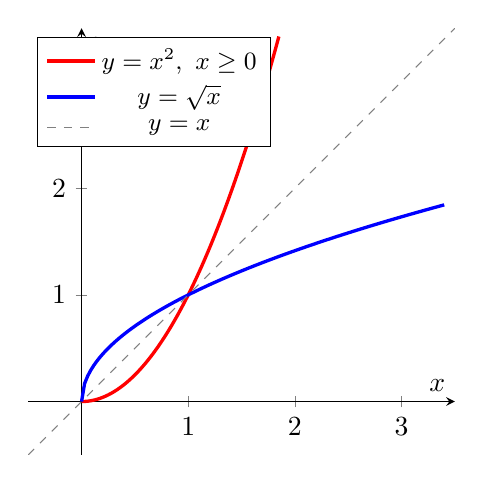
\begin{tikzpicture}
\begin{axis}[
  axis lines=middle, width=7cm, height=7cm,
  xmin=-0.5, xmax=3.5, ymin=-0.5, ymax=3.5,
  xlabel={$x$}, ylabel={$y$}, samples=120,
  legend style={at={(0.02,0.98)},anchor=north west,font=\small}]
\addplot[red, very thick, domain=0:1.85] {x^2};
\addlegendentry{$y=x^2,\ x\ge0$}
\addplot[blue, very thick, domain=0:3.4] {sqrt(x)};
\addlegendentry{$y=\sqrt{x}$}
\addplot[gray, dashed, domain=-0.5:3.5] {x};
\addlegendentry{$y=x$}
\end{axis}
\end{tikzpicture}
\end{center}
Энэ ``мужийг хязгаарлаж урвуу функц гаргах'' санаа Лекц 5-д $\arcsin$, $\arccos$,
$\arctg$ функцүүдийг тодорхойлоход гол үүрэгтэй.
\end{example}

%==============================================================
\section{Графикийн хувиргалт}
%==============================================================
$y=f(x)$ функцийн график мэдэгдэж байг. $a,b\in\R$, $k>0$ байхад:
\begin{center}
\renewcommand{\arraystretch}{1.35}
\begin{tabular}{l|l}
Функц & Графикт хийгдэх хувиргалт \\\hline
$y=f(x-a)$ & $OX$ тэнхлэгийн дагуу $a$-аар шилжинэ \\
$y=f(x)+b$ & $OY$ тэнхлэгийн дагуу $b$-ээр шилжинэ \\
$y=k\,f(x)$ & $OY$ чиглэлд $k$ дахин сунана/шахагдана \\
$y=f(kx)$ & $OX$ чиглэлд $k$ дахин шахагдана/сунана \\
$y=-f(x)$ & $OX$ тэнхлэгийн хувьд тусгал \\
$y=f(-x)$ & $OY$ тэнхлэгийн хувьд тусгал \\
$y=|f(x)|$ & $OX$-ээс доорх хэсгийг дээш тусгана \\
$y=f(|x|)$ & $x\ge0$ хэсгийг үлдээж, $OY$-ийн хувьд тусгана
\end{tabular}
\end{center}

\begin{example}
$y=(x-1)^2-2$ графикийг $y=x^2$ параболыг баруун тийш $1$, доош $2$ шилжүүлж гаргана.
Орой нь $(1,-2)$ цэг.
\end{example}

%==============================================================
\section{Олон гишүүнт ба рационал функц}
%==============================================================

%--------------------------------------------------------------
\subsection{Олон гишүүнт}
%--------------------------------------------------------------
\begin{definition}[Олон гишүүнт]
$a_0,a_1,\ldots,a_n\in\R$, $a_n\neq0$ байхад
\[
P(x)=a_nx^n+a_{n-1}x^{n-1}+\dots+a_1x+a_0
\]
функцийг \itcol{$n$ зэргийн олон гишүүнт} гэнэ. $a_nx^n$-ийг \itcol{ахлах гишүүн},
$a_0$-ийг \itcol{сул гишүүн} гэнэ. $D(P)=\R$.
\end{definition}

\begin{example}
$P(x)=2x^3-4x^2+2$ нь 3 зэргийн олон гишүүнт; ахлах гишүүн $2x^3$, сул гишүүн $2$.

$P(1)=0$ тул $P(x)$ нь $(x-1)$-д хуваагдана:
\[
P(x)=2(x-1)(x^2-x-1).
\]
Иймд $P(x)=0$-ийн шийдүүд $x=1$, $x=\dfrac{1\pm\sqrt5}{2}$ бөгөөд график $OX$ тэнхлэгийг
\[
A\!\left(\tfrac{1-\sqrt5}{2},0\right)\approx(-0.62,\,0),\quad B(1,0),\quad
C\!\left(\tfrac{1+\sqrt5}{2},0\right)\approx(1.62,\,0)
\]
цэгүүдэд огтолно.
\begin{center}
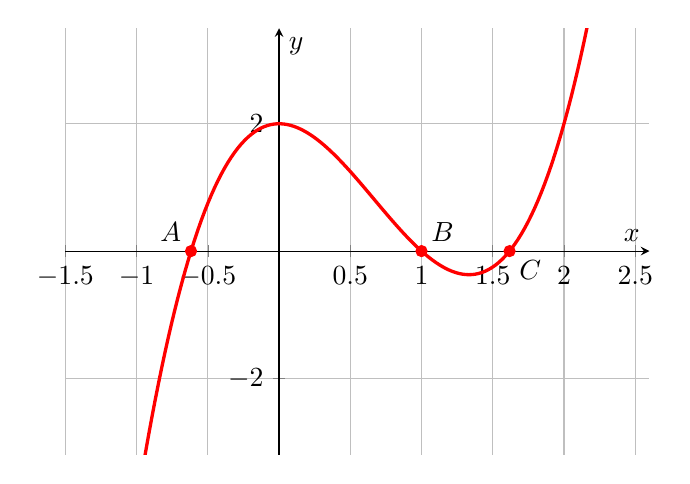
\begin{tikzpicture}
\begin{axis}[
  axis lines=middle, width=9cm, height=7cm,
  xmin=-1.5, xmax=2.6, ymin=-3.2, ymax=3.5,
  xlabel={$x$}, ylabel={$y$}, samples=150, grid=major]
\addplot[red, very thick, domain=-1.1:2.35] {2*x^3-4*x^2+2};
\addplot[red, only marks, mark=*] coordinates {(-0.618,0) (1,0) (1.618,0)};
\node[above left]  at (axis cs:-0.618,0) {$A$};
\node[above right] at (axis cs:1,0) {$B$};
\node[below right] at (axis cs:1.618,0) {$C$};
\end{axis}
\end{tikzpicture}
\end{center}
\end{example}

%--------------------------------------------------------------
\subsection{Рационал функц}
%--------------------------------------------------------------
\begin{definition}[Рационал функц]
$P(x)$, $Q(x)$ олон гишүүнтүүд ($Q\not\equiv0$) бол
\[
f(x)=\frac{P(x)}{Q(x)}
\]
функцийг \itcol{рационал функц} гэнэ. $D(f)=\{x\in\R\mid Q(x)\neq0\}$.
\end{definition}

\begin{example}
$f(x)=\dfrac{x^2-1}{x-2}$.
\begin{itemize}
  \item $x=2$ үед тодорхойлогдохгүй тул $D(f)=(-\infty;2)\cup(2;+\infty)$.
  \item $f(x)=0 \Leftrightarrow x^2-1=0$ тул график $OX$-г $A(-1,0)$, $B(1,0)$ цэгт огтолно.
  \item Хуваалт хийвэл $f(x)=x+2+\dfrac{3}{x-2}$. Иймд $x$ нь $2$-т ойртоход $|f(x)|$
        хязгааргүй өснө ($x=2$ босоо шулуун), $|x|$ ихсэхэд график $y=x+2$ шулуунд
        ойртоно. Эдгээрийг \itcol{асимптот} гэх бөгөөд хязгаарын бүлэгт нарийвчлан үзнэ.
\end{itemize}
\begin{center}
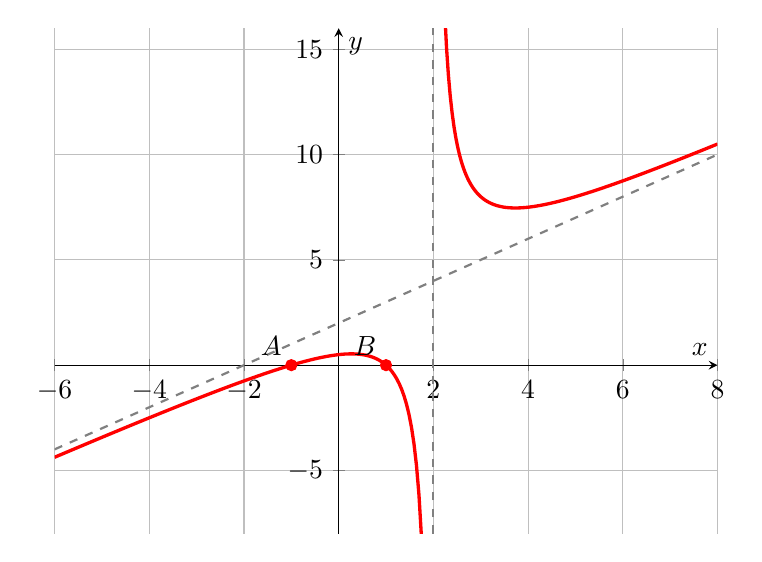
\begin{tikzpicture}
\begin{axis}[
  axis lines=middle, width=10cm, height=8cm,
  xmin=-6, xmax=8, ymin=-8, ymax=16,
  xlabel={$x$}, ylabel={$y$}, samples=150, grid=major]
\addplot[red, very thick, domain=-6:1.8] {(x^2-1)/(x-2)};
\addplot[red, very thick, domain=2.2:8] {(x^2-1)/(x-2)};
\addplot[gray, dashed, thick] coordinates {(2,-8) (2,16)};
\addplot[gray, dashed, thick, domain=-6:8] {x+2};
\addplot[red, only marks, mark=*] coordinates {(-1,0) (1,0)};
\node[above left] at (axis cs:-1,0) {$A$};
\node[above left] at (axis cs:1,0) {$B$};
\end{axis}
\end{tikzpicture}
\end{center}
\end{example}

%##############################################################
\section{Семинар ба гэрийн даалгавар (Лекц 4)}
%##############################################################

%--------------------------------------------------------------
\subsection*{A. Функцийн ангилал ба нийлмэл функц}
%--------------------------------------------------------------
\begin{enumerate}
\item Дараах функцүүдийг $f=g\circ h$ хэлбэрээр бич.
\begin{enumerate}
  \item $f(x)=|x^2-1|$
  \item $f(x)=\sqrt{1-x^2}$
  \item $f(x)=e^{-x^2}$
  \item $f(x)=\cos 2x$
  \item $f(x)=(3x-1)^4$
  \item $f(x)=\ln(x^2+1)$
  \item $f(x)=\arctg(2x)$
  \item $f(x)=\sqrt{\sin x}$
\end{enumerate}
\item Дараах функцүүдийг $f=g\circ h\circ s$ хэлбэрээр бич.
\begin{enumerate}
  \item $f(x)=\dfrac{1}{\sqrt{1-x^2}}$
  \item $f(x)=\dfrac{1}{1+e^{-x}}$
\end{enumerate}
\item Дурын $f:\R\to\R$ функцийг тэгш ба сондгой функцийн нийлбэрт задалж болно гэж батал.
      \textit{(Зөвлөмж: $\frac{f(x)+f(-x)}{2}$ ба $\frac{f(x)-f(-x)}{2}$.)} $e^x$-ийн хувьд задал.
\end{enumerate}

%--------------------------------------------------------------
\subsection*{B. Олон гишүүнт ба биномын томьёо}
%--------------------------------------------------------------
\begin{theorem}[Биномын томьёо]
$n\in\N$ бол
\[
(a+b)^n=\sum_{k=0}^{n}\binom{n}{k}a^{n-k}b^k,\qquad \binom nk=\frac{n!}{k!(n-k)!}.
\]
Жишээ нь $(a+b)^3=a^3+3a^2b+3ab^2+b^3$.
\end{theorem}

\begin{enumerate}[resume]
\item $(1+x)^5$-ийг задалж, $x^3$-ийн коэффициентийг ол.
\item $(x^2+3x)^3$-ийг задлаад $x^4$-ийн коэффициентийг ол.
\item $x^4+x^3-x^2+x-2$-ийг үржигдэхүүнд задал.
\end{enumerate}

%--------------------------------------------------------------
\subsection*{C. Утгын муж}
%--------------------------------------------------------------
\begin{enumerate}[resume]
\item Дараах функцүүдийн утгын мужийг ол.
\begin{enumerate}
  \item $f(x)=\sqrt{8-2x-x^2}$
  \item $f(x)=\sqrt{2x-1-x^2}$
  \item $f(x)=1-\sqrt{9-\sqrt{2x^2+6\sqrt2x+9}}$
  \item $f(x)=\begin{cases}2x^2+8x+6, & x<-1,\\ 3\sqrt{x+1}, & x\ge-1\end{cases}$
  \item $f(x)=\begin{cases}\dfrac8x, & x\le-2,\\ x^3+4, & -2<x\le0,\\ \dfrac{4}{x^2+1}, & x>0\end{cases}$
  \item $f(x)=\dfrac{x^4+6x^3-27x-162}{x^2+3x-18}$
\end{enumerate}
\end{enumerate}

%--------------------------------------------------------------
\subsection*{D. Урвуу функц}
%--------------------------------------------------------------
\begin{enumerate}[resume]
\item Урвуу функцийг ол.
\begin{enumerate}
  \item $y=x|x|+2x$, \; $x\in\R$
  \item $y=\dfrac{x^2+1}{2x}$, \; $x\in[1;+\infty)$
  \item $y=\dfrac{x^2+1}{2x}$, \; $x\in(0;1]$
  \item $y=x-\sqrt{x^2-1}$, \; $x\in(-\infty;-1]$
\end{enumerate}
\end{enumerate}

%--------------------------------------------------------------
\subsection*{E. График}
%--------------------------------------------------------------
\begin{enumerate}[resume]
\item $f(x)=\dfrac{x^2-1}{x+1}$ функцийн графикийг зур. ($x=-1$ цэгт юу болохыг анхаар.)
\end{enumerate}

\begin{enumerate}[resume]
\item Дараах функцүүдийн графикийг дүрсэл.
\begin{enumerate}
  \item $f(x)=\begin{cases}1, & x>0,\\ 0, & x=0,\\ -1, & x<0\end{cases}$
  \item $f(x)=\begin{cases}x+1, & x>0,\\ x-1, & -1\le x<0,\\ x^2-1, & x<-1\end{cases}$
  \item $f(x)=\sqrt{x^2+2x+1}+\sqrt{x^2-4x+4}$
  \item $f(x)=(x-1)(1-x^4)(x+2)^2$
  \item $f(x)=\dfrac{(x-4)(x^2-9)}{x^2-5x+6}$
\end{enumerate}
\end{enumerate}